\iffalse
\documentclass{article}
\usepackage{amsmath}
\usepackage{xcolor}
\usepackage{gensymb}
\usepackage{ragged2e}
\usepackage{graphicx}
\usepackage{gensymb}
\usepackage{mathtools}
\newcommand{\mydet}[1]{\ensuremath{\begin{vmatrix}#1\end{vmatrix}}}
\providecommand{\brak}[1]{\ensuremath{\left(#1\right)}}
\providecommand{\norm}[1]{\left\lVert#1\right\rVert}
\newcommand{\solution}{\noindent \textbf{Solution: }}
\newcommand{\myvec}[1]{\ensuremath{\begin{pmatrix}#1\end{pmatrix}}}
\let\vec\mathbf 


\begin{document}
\begin{center}
        \textbf\large{CHAPTER-7 \\ TRIANGLES}
\end{center}
\section{Exercise 7.1}
Q3. 
\textbf{Construction}\\
\fi
See 
	\figref{fig:chapters/9/7/1/3/Fig1}
\begin{figure}[h]
	\begin{center}
		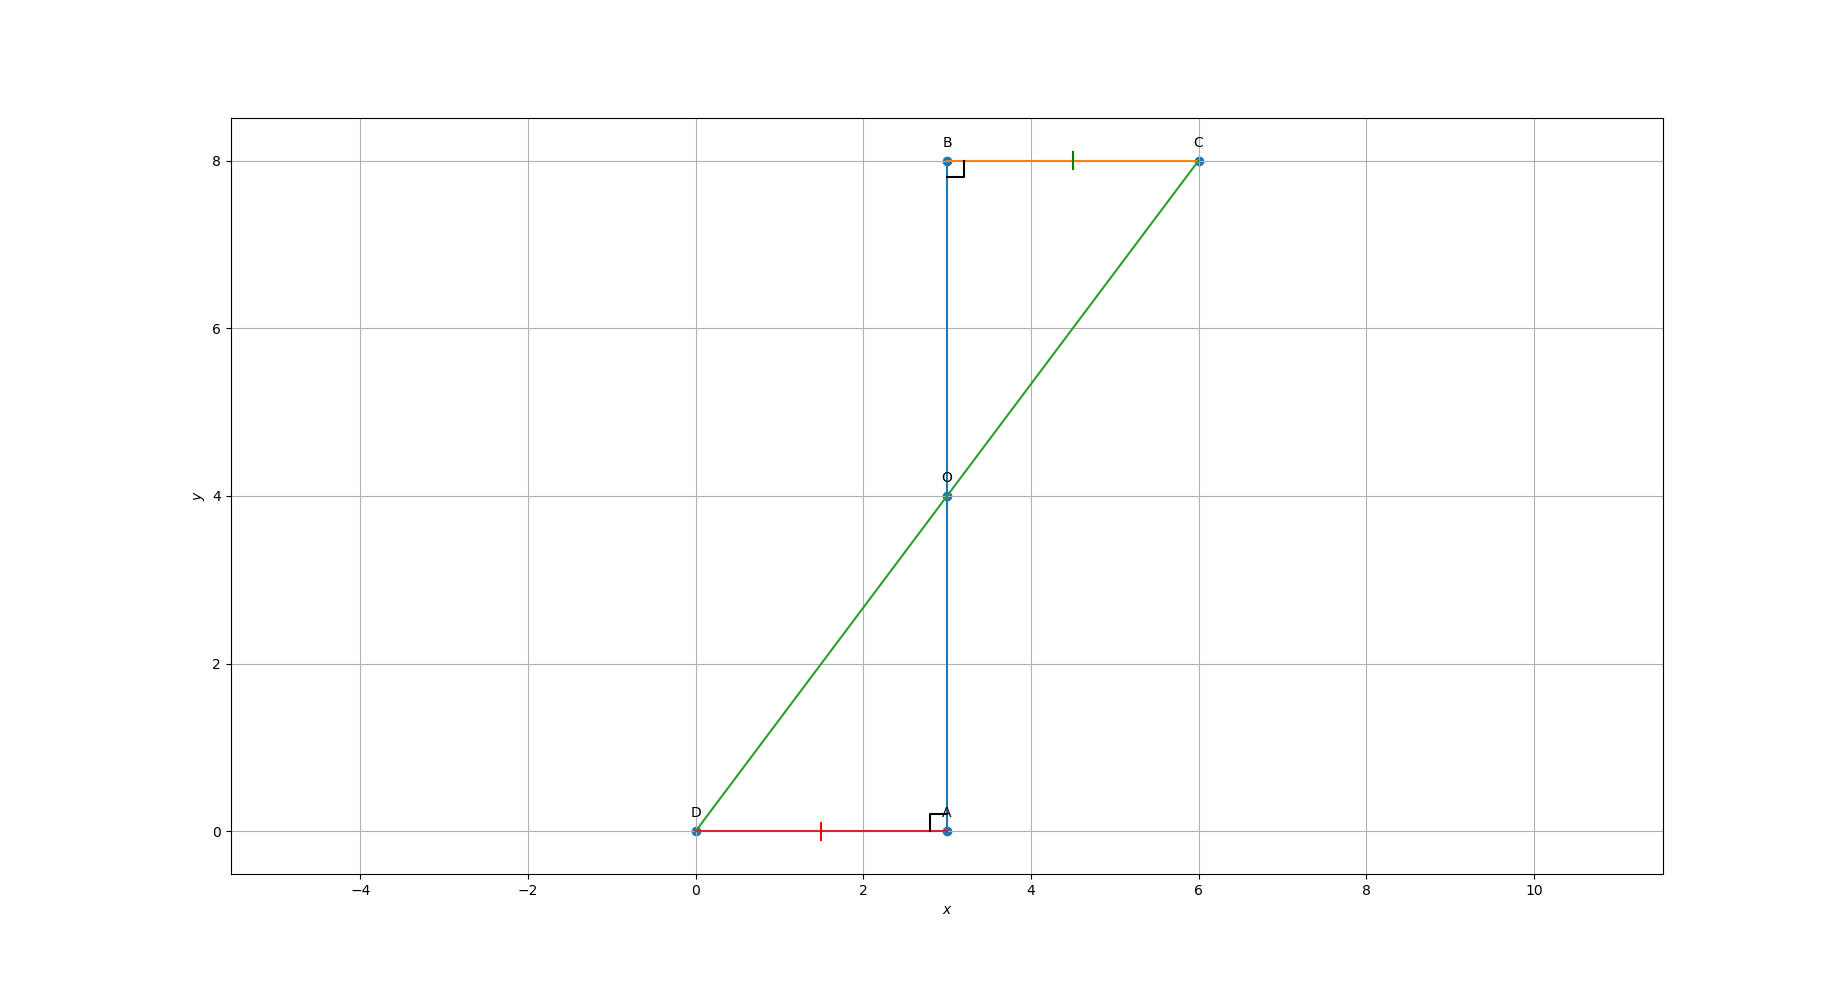
\includegraphics[width=\columnwidth]{chapters/9/7/1/3/figs/Figure1.png}
	\end{center}
	\caption{}
	\label{fig:chapters/9/7/1/3/Fig1}
\end{figure}
The input parameters for construction are shown in \tabref{tab:chapters/9/7/1/3/Table1}
\begin{table}[h]
	  \centering
	  \begin{tabular}{|p{3cm}|p{3cm}|p{3cm}|}
\hline                                        
	\textbf{Symbol} & \textbf{Values} & \textbf{Description} \\                                          
\hline                                 
	a & 3 & $AD=BC$ \\        
\hline                                    
	b & 8 & $AB$ \\    
\hline                      
	$\vec{e}_1$ & $\myvec{1\\0}$ & basis vector \\
\hline
\end{tabular}

	  \caption{Parameters}
	  \label{tab:chapters/9/7/1/3/Table1}
\end{table}
Let
\begin{align}
	\vec{A} = a\vec{e_1},\vec{B} = \myvec{a\\b},\vec{C} = \myvec{2a\\b},\vec{D} = \myvec{0\\0}
\end{align}
\solution
Given
\begin{align}
	\norm{\vec{D}-\vec{A}}&=\norm{\vec{B}-\vec{C}}
	\\
	\angle DAB &= \angle CBA=90\degree
\end{align}
\begin{align}
	\frac{1}{2}(\vec{C}+\vec{D}) &= \frac{1}{2}\myvec{a \\ \frac{b}{2}}
	\\
	\frac{1}{2}(\vec{A}+\vec{B}) &= \frac{1}{2}\myvec{a \\ \frac{b}{2}}
		 \label{eq:chapters/9/7/1/3/1}\\
\end{align}
Thus, $CD$ bisects $AB$.
